
\section*{Makeham and Gompertz survival distributions}

\subsection*{Q1}

Let $Y = \log(1+\frac{V \log(c)}{b}) / \log(c) = \log_c(1+\frac{V \log(c)}{b})$ and $V \sim \text{exponential}(1)$. Then a straightforward calculation gives the result:
\begin{equation}
c^Y - 1 = c^{ \log_c(1+\frac{V \log(c)}{b})} - 1 = 1+\frac{V\log(c)}{b} - 1 = \frac{V \log(c)}{b}
\end{equation}

and because $V \sim \text{exponential}(1)$ we have that

\begin{equation}
\Pr[c^Y - 1 \le x ] = \Pr[V \frac{\log(c)}{b} \le x ] = \Pr[V \le x \frac{b}{\log{c}}] 
\end{equation}
so that $c^Y - 1 \sim \text{exponential}( \frac{b}{\log(c)})$. Then using the explicit form of the CDF of the exponential distribution we find using $Z = c^Y - 1 $
\begin{equation}
\begin{split}
\Pr[Y > x] & = \Pr[c^Y - 1 > c^x - 1] \\ 
		 & = \Pr[Z > c^x - 1] = 1- \Pr[Z \le c^x - 1]  \\
		 & = 1 - F_Z(c^x - 1) = 1 - (1-\exp(-\frac{b}{\log c} (c^x - 1))) \\
	     & = \exp(-\frac{b}{\log c} (c^x - 1))
\end{split}
\end{equation}
which is equal to equation (2) from the exercises with $a = 0$ so $ Y \sim \text{Gompertz}(b,c)$.

\subsection*{Q2}
If the code is entered into \verb|R| we obtain the following results
\begin{verbatim}
> gen.Sample <- function(n, a, b, c)
+ {if (any(a<0,b<0,c<1)) stop("Invalid parameters")
+   lifetimes <- log(1+rexp(n)*log(c)/b)/log(c)
+   if (a>0) lifetimes <- pmin(lifetimes, rexp(n)/a)
+   return(lifetimes)}
> set.seed(2525); G <- gen.Sample(2000, 0, 8e-5, 1.08)
> set.seed(2525); M <- gen.Sample(2000, 5e-4, 8e-5, 1.08)
> all(G>=M) 
[1] TRUE
> mean(M==G) 
[1] 0.959
> rbind(Gompertz=summary(G), Makeham=summary(M))
           Min. 1st Qu. Median  Mean 3rd Qu.  Max.
Gompertz 4.9450   73.72  85.12 81.98   93.73 116.6
Makeham  0.2809   71.85  84.15 80.08   93.35 116.6
\end{verbatim}

Since the Makeham distribution is defined as $X = min(Y,Z)$ with $Y \sim \text{Gompertz}(b,c)$ and $Z \sim \text{exponential}(a)$ the results of the Makeham distribution are always smaller or equal to the Gompertz results. This is verified by the result \verb+all(G>M)+ is TRUE. \\
The result of \verb+mean(M==G)+ is 0.959 which implies that in 95,9\% of the cases the cause of death is equal to the Gompertz results. The probability of dying of old ages with these parameters is therefore 0.959.

\subsection*{Q3}
We run the code to assess the effect of changes on the parameters on the mean life-time and obtain the following result
\begin{verbatim}
> S <- function(x, a, b, c) exp(-a*x - b/log(c)*(c^x-1))
> a <- 5e-4; b <- 8e-5; c <- 1.09
> mean.age <- integrate(S, 0, Inf, a, b, c)$value 
> mean(gen.Sample(1e6, a, b, c))
[1] 73.00126
> integrate(S, 0, Inf, 1.02*a, b, c)$value / mean.age
[1] 0.9996164
> integrate(S, 0, Inf, a, 1.02*b, c)$value / mean.age
[1] 0.9969848
> integrate(S, 0, Inf, a, b, 1.02*(c-1)+1)$value / mean.age
[1] 0.9844023
> 
\end{verbatim}
The results imply that a 2\% increase in the parameter a leads to a very small percentage decline of the mean life-time of approximately 0.04\%. The impact of a 2\% increase in the b parameter leads to a slightly larger decrease on the mean life-time of approximately 0.3\%. The impact of the scaling of the c parameter leads to approximately a 1.6\% decrease of the mean life-time. Increasing the paramters therefore leads to an increase in mortality.

\subsection*{Q4}

By using the logarithm of the likelihood function we evade the problem of limited machine precision. If we let \verb|R| calculate the a few exponentials we obtain the following output

\begin{verbatim}
> exp(-8300)
[1] 0
> exp(-10000)
[1] 0
> exp(-5000)
[1] 0
> exp(-100)
[1] 3.720076e-44
> exp(-10)
[1] 4.539993e-05
> 
\end{verbatim}

which implies that \verb|R| does not have the capacity to differentiate between the numbers $\exp{(-10000)}$, $\exp{(-8300)}$ and $\exp{(-5000)}$ for example. Only if the exponent is sufficiently small \verb|R| will have the ability to differentiate between the numbers and find an optimum. By passing to the logarithm of the likelihood function we circumvent this problem. 


\subsection*{Q5}

To obtain ML-estimates for the M sample the code given in the exercise gives the following output:
\begin{verbatim}
> log.Lik <- function(p) {- sum(log.fx(M, p[1], p[2], p[3]))} ## Makeham on Makeham
> a <- 5e-4; b <- 8e-5; c <- 1.08
> oMM <- optim(c(a,b,c), log.Lik) 
There were 26 warnings (use warnings() to see them)
> oMM$value ## 8428.489
[1] 8428.489
> oMM$par ## a=7.3e-04 b=6.0e-05 c=1.083
[1] 7.338301e-04 5.993626e-05 1.083515e+00
> 
> log.Lik <- function(p) {-sum(log.fx(M, 0, p[1], p[2]))} ## Gompertz on Makeham
> a <- 0; b <- 8e-5; c <- 1.08
> oGM <- optim(c(b,c), log.Lik) ## 13x NaN
There were 13 warnings (use warnings() to see them)
> oGM$value ## 8456.258
[1] 8456.258
> oGM$par ## a=0 b=1.3e-4 c=1.074
[1] 0.0001292634 1.0741178742
>
\end{verbatim}

To find the ML-estimates for the G sample we use a similar code and obtain

\begin{verbatim}
> log.Lik <- function(p) {-sum(log.fx(G, p[1], p[2], p[3]))} ## Makeham on Gompertz
> a <- 5e-4; b <- 8e-5; c <- 1.08
> oMG <- optim(c(a,b,c), log.Lik) ## 13x NaN
There were 33 warnings (use warnings() to see them)
> oMG$value
[1] 8245.877
> oMG$par
[1] 1.585592e-04 5.928508e-05 1.083783e+00
> 
> log.Lik <- function(p) {-sum(log.fx(G,0, p[1], p[2]))} ## Gompertz on Gompertz
> a <- 0; b <- 8e-5; c <- 1.08
> oGG <- optim(c(b,c), log.Lik) ## 13x NaN
There were 13 warnings (use warnings() to see them)
> oGG$value
[1] 8248.117
> oGG$par
[1] 7.088547e-05 1.081598e+00
>
\end{verbatim}

Summarizing the output we have the following results 

\begin{center}

\begin{tabular}{r | r | r | r | r}
 							 & a & b & c & ML \\ \hline
 Makeham on Makeham sample 	 & 7.338301e-04 & 5.993626e-05 & 1.083515e+00 & 8428.489 \\
 Gompertz on Makeham sample  & 0 & 0.0001292634 & 1.0741178742 & 8456.258 \\
 Makeham on Gompertz sample  & 1.585592e-04 & 5.928508e-05 & 1.083783e+00 & 8245.877 \\
 Gompertz on Gompertz sample & 0 & 7.088547e-05 & 1.081598e+00 & 8248.117 
 
\end{tabular}

\end{center}

\subsection*{Q6}

We have the following formulas for the AIC
\begin{equation}
AIC = -2 \log L + 2k
\end{equation}
and for the BIC criteria 
\begin{equation}
BIC = -2 \log L + k \log n \approx -2 \log L + 7.6k
\end{equation}
where the approximation is for the current situation. For the Makeham model there are 3 parameters ($k = 3$) and for the Gompertz model there are 2 parameters ($k=2$).

Via \verb|R| we compute the values for the AIC and BIC criteria in the optima for the different situations and test if the Makeham model has a smaller AIC or BIC and obtain the output
\begin{verbatim}
> AIC.MM <- 2*oMM$value + 2 * 3;
> AIC.GM <- 2*oGM$value + 2 * 2;
> AIC.MG <- 2*oMG$value + 2 * 3;
> AIC.GG <- 2*oGG$value + 2 * 2;
> 
> BIC.MM <- 2*oMM$value + 7.6 * 3;
> BIC.GM <- 2*oGM$value + 7.6 * 2;
> BIC.MG <- 2*oMG$value + 7.6 * 3;
> BIC.GG <- 2*oGG$value + 7.6 * 2;
> 
> (AIC.MM<AIC.GM)
[1] TRUE
> (AIC.MG<AIC.GG)
[1] TRUE
> (BIC.MM<BIC.GM)
[1] TRUE
> (BIC.MG<BIC.GG)
[1] FALSE
> \end{verbatim}

As regards to AIC the Makeham model is better on both samples. As regards to the BIC the Makeham model is better on the Makeham sample but the Gompertz model is better on the Gompertz sample.

\subsection*{Q7}

If the following code is submitted in \verb|R|

\begin{verbatim}
S <- function(x, a, b, c) exp(-a*x - b/log(c)*(c^x-1))
x <- 0:110
plot(x, 1-S(x, 0, 8e-5, 1.08), type="h", ylab="F(x; a,b,c)")
lines(x, 1-S(x, 1e-3, 8e-5, 1.08), col="red")
points(x, 1-S(x, 0, 8e-5, 1.09), col="blue")
\end{verbatim}
\verb|R| generates the plot as seen in Figure \ref{Figure_Question7}.

\begin{center}
\begin{figure}[H]

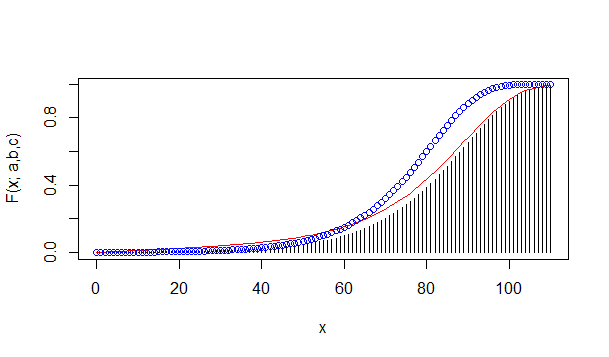
\includegraphics[scale=1]{Question_7_MakehamGompertz.png}

\caption{The bar chart describes a Gompertz distribution with $b = 8 \cdot 10^{-5}$ and $c=1.08$. The red line is a Makeham distribution with $a=1\cdot 10^{-3}$ and $b, c$ equal to the Gompertz distribution. The blue dots represent the Gompertz distribution with the parameter $c = 1.09$.}
\label{Figure_Question7}

\end{figure}
\end{center}

The difference between the Gompertz (bars in Figure \ref{Question_7_MakehamGompertz}) and Makeham distribution (red line) can clearly be seen in the figure. Since Makeham also has a 'accident' part in the model the cdf shows higher probabilities at low ages. For old ages the two distribution converge and are appoximately equal. The blue dots represent a Gompertz distribution with a higher parameter $c$. The effect of increasing the $c$ parameter leads to an increase in the cdf especially for older ages.


\subsection*{Q8}

If the following code is submitted in R

\begin{verbatim}
mu <- function(x, a, b, c) (a + b*c^x)
x <- 0:110
plot(x, mu(x, 0, 8e-5, 1.08), type="h", ylab="F(x; a,b,c)")
lines(x, mu(x, 1e-3, 8e-5, 1.08), col="red")
points(x, mu(x, 0, 8e-5, 1.09), col="blue")
\end{verbatim}

the output from \verb|R| is given in figure \ref{Figure_Question8}.
\begin{center}
\begin{figure}[H]

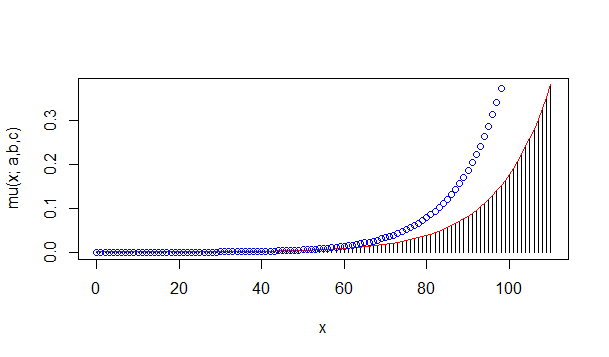
\includegraphics[scale=1]{Question_8_MakehamGompertz.png}

\caption{The bar chart describes the mortality rate for Gompertz' law with $b = 8 \cdot 10^{-5}$ and $c=1.08$. The red line is the Makeham extension with $a=10^{-3}$ and $b,c$ equal to the Gompertz case. The blue dots represent the Gompertz case with the parameter $c = 1.09$.}
\label{Figure_Question8}

\end{figure}
\end{center}

The Makeham mortality rate with $a = 10^{-3}$ is almost indistinguishable from the Gompertz mortality rate. Changing the parameter $c$ to $1.09$ has a large impact on the mortality rate. At ages higher than 70 years old the mortality rate increases dramatically.


\subsection*{Q9}

Since $q_x = \frac{S(x-1) - S(x)}{S(x-1)}$ we can fill the dots in the code in the following way using the \verb+diff(c)+ and \verb+head()+ functions and optimize. We obtain the following output

\begin{verbatim}
> S <- function(x, a, b, c) exp(-a*x - b/log(c)*(c^x-1))
> agerange <- 1:nages ## denotes the range of ages accounted for when finding ML
> LogLik <- function(p)
+ { ddfs <- S(0:nages, p[1], p[2], p[3])
+ q.x <- -diff(ddfs)/head(ddfs,nages)
+ -sum(dbinom(D.x[agerange], e.x[agerange], q.x[agerange], log=TRUE))}
> a <- 1e-4; b <- 8e-5; c <- 1.08
> o <- optim(c(a,b,c), LogLik) 
There were 16 warnings (use warnings() to see them)
> o$value
[1] 191373.5
> o$par
[1] 9.206514e-04 1.844402e-05 1.113540e+00
>
\end{verbatim}
so the ML-estimates for $a, b$ and $c$ are $a = 1.077 \cdot 10^{-3}, b=1,433 \cdot 10^{-6}$ and $c = 1.166$. \\
Submitting the code
\begin{verbatim}
ddfs <- S(0:nages, o$par[1], o$par[2], o$par[3])
q.x <- -diff(ddfs)/head(ddfs,nages)

plot(1:nages,D.x[1:nages]/e.x[1:nages],type="p",
     main="Optimally estimated qx & fractions Dx/ex",xlab="age",ylab="q_x")
lines(1:nages, q.x[1:nages], col="blue")
\end{verbatim}
gives the plot in figure \ref{Figure_Question9_1}.
\begin{center}
\begin{figure}[H]

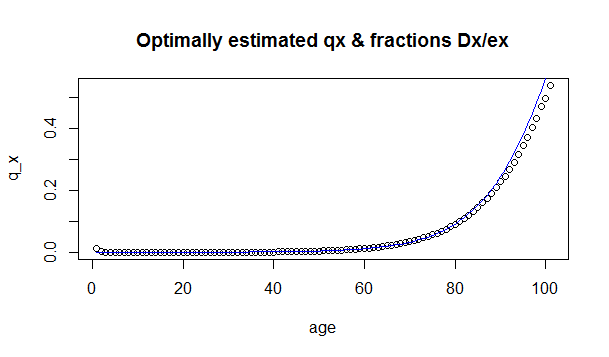
\includegraphics[scale=1]{Question_9_MakehamGompertz_1.png}

\caption{Plot of the ML estimate and the fractions $D_x/e_x$}
\label{Figure_Question9_1}

\end{figure}
\end{center}

The Makeham fit is not valid for ages in $(0,1]$ and the expectation is that the estimation is better when $x=1$ is left out. If we run the following code in \verb|R| we obtain the result without $x=1$.
\begin{verbatim}

> S <- function(x, a, b, c) exp(-a*x - b/log(c)*(c^x-1))
> agerange <- 2:nages ## denotes the range of ages accounted for when finding ML
> LogLik <- function(p)
+ { ddfs <- S(0:nages, p[1], p[2], p[3])
+ q.x <- -diff(ddfs)/head(ddfs,nages)
+ -sum(dbinom(D.x[agerange], e.x[agerange], q.x[agerange], log=TRUE))}
> a <- 1e-4; b <- 8e-5; c <- 1.08
> o2 <- optim(c(a,b,c), LogLik) 
There were 20 warnings (use warnings() to see them)
> o2$value
[1] 15217.31
> o2$par
[1] 0.0004726379 0.0000246149 1.1095517146
> 
> ddfs <- S(0:nages, o2$par[1], o2$par[2], o2$par[3])
> q2.x <- -diff(ddfs)/head(ddfs,nages)
> 
> plot(1:nages,D.x[1:nages]/e.x[1:nages],type="p",
+      main="Optimally estimated qx & fractions Dx/ex",xlab="age",ylab="q_x")
> lines(1:nages, q.x[1:nages], col="blue")
> lines(1:nages, q2.x[1:nages], col="red")
>
\end{verbatim}

and the plot in figure \ref{Figure_Question9_2}.

\begin{center}
\begin{figure}

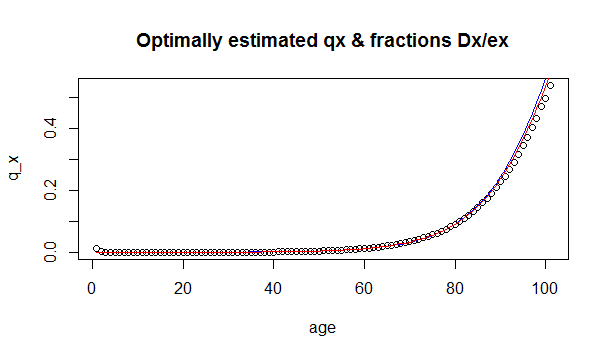
\includegraphics[scale=1]{Question_9_MakehamGompertz_2.png}

\caption{Plot of the ML estimate (blue line), the fractions $D_x/e_x$ and ML estimate without $x=1$ (red line)}
\label{Figure_Question9_2}

\end{figure}
\end{center}
Clearly the fit without $x=1$ is better (red line in figure) for high ages.

To investigate the 'accident hump' we plot \verb+q.x[1:60]+ (with and without $x=1$) and \verb+(D.x/e.x)[1:60]+. Submitting the following code

\begin{verbatim}
nages <- 60
plot(1:nages,D.x[1:nages]/e.x[1:nages],type="p",
     main="Optimally estimated qx & fractions Dx/ex",xlab="age",ylab="q_x")
lines(1:nages, q.x[1:nages], col="blue")
lines(1:nages, q2.x[1:nages], col="red")
\end{verbatim}

gives the plot shown in figure \ref{Figure_Question9_3}.
\begin{center}
\begin{figure}
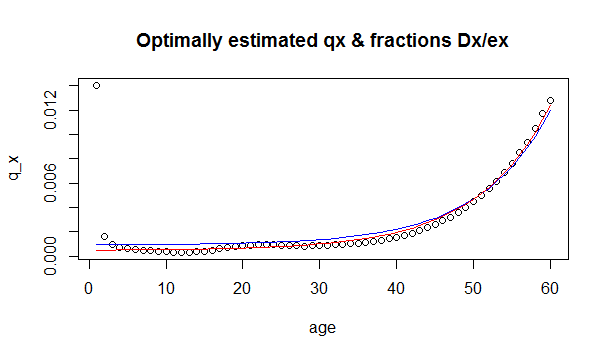
\includegraphics[scale=1]{Question_9_MakehamGompertz_3.png}
\caption{Plot of the ML estimate (blue line), the fractions $D_x/e_x$ and ML estimate without $x=1$ (red line) for $ x \in [0,60]$.}
\label{Figure_Question9_3}
\end{figure}
\end{center}		

The figure clearly shows the accident hump at $x=20$. 

